%kelompok 1 Sistem Operasi (Semaphore)
%Kelas D4 TI 1B
%Adam Noer Hidayatullah 1174097
%Ichsan Hizman
%Teddy
%Nisrina Aulia
%Irvan Rizkiansyah 1174043

\section{proses}

	\subsection{Proses}	
	Proses adalah sebuah  program yang sedang dieksekusi. Sedangkan program adalah kumpulan-kumpulan  suatu  instruksi yang sudah  ditulis ke dalam bahasa yang dimengerti sistem operasi.Proses berisi tentang  sebuah instruksi dan sebuah  data. program counter dan seluruh register pemroses, stack ini  berisi data sementara contoh  seperti parameter rutin, alamat pengiriman dan variabel lokal.Sistem operasi harus mengelola semua proses di dalam sistem tersebut dan mengalokasikan sumber daya ke sebuah  proses-proses sesuai dengan kebijaksanaan untuk memenuhi sasaran sistem
	
	\subsection{Istilah yang berkaitan dengan proses}
		\begin{itemize}
			\item Multiprogramming
			Multiprogramming (multitasking) adalah  istilah teknologi informasi dengan mengunakan bahasa inggris yang baik  mengacup kepada sebuah metode dimana banyak sebuah pekerjaan atau yang dikenal juga sebagai proses  dengan diolah dengan menggunakan sumber daya CPU yang sama.
			Contohnya sistem operasi jenis ini antaranya linux dan windows.
			\item Multiprocessing
			kemampuan komputer untuk melakukan beberapa proses dengan waktu yang bersamaan, dibantu dengan keberadaan teknologi yang berbasis multiprocessor.
			Contohnya seperti computer server.
			\item Distributed processing/computing
			Mengerjakan semua proses pengolahan data secara bersamaan antara komputer pusat dengan beberapa komputer yang lebih kecil dan saling berhubungan denan melalui jalur komunikasi.
			Contohnya komputer yang dirancang untuk melaksanakan tugas-tugas proyek.
		\end{itemize}
		
	\subsection{Status proses}
	Terdapat 5 macam jenis status yang mungkin dimiliki oleh suatu proses :
	\begin{enumerate}
		\item New, yaitu status yang dimiliki pada saat proses baru saja terjadi.
		\item Ready, yaitu status dimana proses siap untuk dieksekusi pada giliran berikutnya.
		\item Running, yaitu status dimana saat ini proses sedang dieksekusi oleh prosesor
		\item Waiting, yaitu status dimana proses yang tidak bisa dijalankan di saat prosesor sudah siap, status yang dimiliki pada saat proses menunggu suatu sebuah event seperti I/O
		\item Terminated, yaitu status yang dimiliki pada saat proses telah selesai dieksekusi
	\end{enumerate}
	
	Berikut ini adalah proses dari ke-5 status proses di atas :
	\begin{enumerate}
		\item New ke Ready
		Pertama Status dibuat lalu setelah itu , status akan memasuki proses ready dan siap untuk memasuki proses selanjutnya.
		\item Ready ke running
		Di saat sedang memilih proses yang akan dioperasikan, sistem operasi akan memilih salah satu proses yang berada didalam keadaan status ready.
		\item Running ke waiting
		Suatu proses dimasukkan dalam keadaan status waiting jika proses itu meminta sesuatu yang dapat menyebabkannya harus menunggu. Sebuah request ke sistem operasi pada umumnya merupakan bentuk panggilan dari layanan sistem (panggilan dari program yang sedang beroperasi ke prosedur yang sedang beroperasi ke prosedur yang merupakan bagian kode sistem operasi) misalnya seperti sebuah proses bisa meminta suatu layanan dari sistem operasi yang tidak siap dilakukan sistem opersi dengan segera. Atau proses dapat menginisiasi suatu aksi, misalnya operasi I/O, yang harus diselesaikan sebelum proses itu melanjutkan operasinya. Pada saat proses saling berkomunikasi dengan proses lainnya, suatu proses bisa diblokir jika sedang menunggu proses lainnya untuk menyediakan input atau sedang menunggu pesan dari proses lainnya.
		\item Running ke ready
		Pada umumnya alasan transisi ini ialah dimana sebuah proses yang lagi berjalan sudah mencapai batas waktu maksimum yang telah diizinkan bagi instruksi yang tidak diinterupsi. Terdapat beberapa alasan yang menyebabkan transisi ini terjadi, yang tidak diimplementasikan oleh setiap sistem operasi. Misalnya apabila sistem operasi meng-assign tingkat prioritas yang berbeda pada beberapa proses yang berlainan, suatu proses bisa diambil lebih dulu.
		\item Waiting ke ready
		Apabila suatu proses dalam keadaan status waiting sudah selesai dalam mendapatkan sumber daya, seperti file atau bagian virtual memori bagi pakai atau juga sudah selesai setelah menunggu proses yang lainnya untuk menyediakan input atau sudah selesai dalam menunggu pesan lainnya.
		\item Runing ke finish(terminated)
		proses yang sedang berjalan dihentikan oleh Sistem Operasi jika proses itu telah selesai atau tidak jadi dieksekusi. Hal ini terjadi dikarenakan jika proses induknya sendiri telah berhenti.
	\end{enumerate}
	
	Dan berikut ini adalah diagram dari ke-5 status proses tadi :
	
	\begin{figure} [ht]
	\centerline{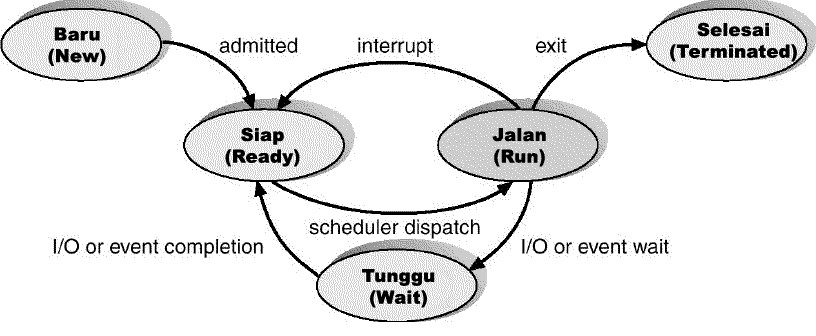
\includegraphics[width=1\textwidth]{figures/statusproses.jpg}}
	\caption{Gambar Status Proses}
	\label{statusproses}
	\end{figure}
	
	\ref{statusproses}